% Created 2018-08-24 Fri 09:05
% Intended LaTeX compiler: pdflatex
\documentclass[final]{beamer}
	         \usetheme{ph}
           \usepackage[orientation=portrait,size=a0,scale=1.4]{beamerposter}
           \usepackage[absolute,overlay]{textpos}
	         \usepackage[authoryear]{natbib}


\setlength{\paperwidth}{36in}
\setlength{\paperheight}{55in}
\setlength{\textwidth}{0.98\paperwidth}
\setlength{\textheight}{0.98\paperheight}
\graphicspath{{../output/figures/}{../lib/}}
\usepackage[export]{adjustbox}
\usepackage{graphicx,caption}
\usepackage{minted}
\usepackage{eurosym}
\usepackage{listings}
\usepackage{textcomp}
\usepackage{bibentry}
\usepackage{tikz}
\usetikzlibrary{positioning,shapes.geometric}
\input{\string~/.emacs.d/misc/GrandMacros}
\date{}
\newcommand{\auth}{Kazuki Yoshida, MD, MPH, MS}
\newcommand{\authemail}{kazukiyoshida@mail.harvard.edu}
\newcommand{\authtwitter}{@kaz\_yos}
\newcommand{\authgithub}{github.com/kaz-yos}
\author{
Kazuki Yoshida$^{1,2}$
Daniel H Solomon$^{2}$
Sebastien Haneuse$^{1}$
Seoyoung C Kim$^{2}$
Elisabetta Patorno$^{2}$ \\
Sara K Tedeschi$^{2}$
Houchen Lyu$^{2}$
Sonia Hernandez-Diaz$^{1}$
Robert J Glynn$^{1,2}$
\\
\normalsize{$^{1}$ Harvard T.H. Chan School of Public Health, Boston, MA, USA; }
\normalsize{$^{2}$ Brigham and Women's Hospital, Boston, MA, USA}
}
\usetheme{default}
\date{2018-08-24 09:05}
\title{Multinomial Extension of Propensity Score Trimming Methods: A Simulation Study}
\begin{document}

\begin{frame}[label={sec:org6cddcf1}]{}
\vspace{-1cm}
\begin{columns}
\begin{column}[t]{0.48\columnwidth}
\begin{block}{Conflict of Interest}
\small
KY received support from Harvard T.H. Chan School of Public Health (partially supported by Pfizer, Takeda, Bayer and ASISA) and Honjo International Scholarship Foundation. DHS receives salary support from institutional research grants from Eli Lilly, Amgen, Pfizer, AstraZeneca, Genentech, and Corrona. He also receives royalties from UpToDate, and serves in unpaid roles in studies funded by Pfizer and Eli Lilly. RJG received research support in the form of grants to his institution from AstraZeneca, Kowa, Novartis, and Pfizer. Other authors declared no COI.
\end{block}


\begin{block}{Background}
\large
\begin{itemize}
\item \cite{crump_dealing_2009}, \cite{sturmer_treatment_2010} and \cite{walkerToolAssessingFeasibility2013} have proposed propensity score (PS) trimming methods for binary exposures.

\item \cite{sturmer_treatment_2010} demonstrated benefits of PS trimming in reducing unmeasured confounding in the presence of unmeasured confounders that were more prevalent in the tails of the PS distribution.

\item We extended binary PS trimming methods to the general multinomial settings. We illustrated and examined their characteristics in the visually-tractable 3-group setting.
\end{itemize}
\end{block}


\begin{block}{Notations}
\small
\begin{center}
\begin{tabular}{ll}
Notation & Explanation\\
\hline
\(i \in \left\{ 1,...,n \right\}\) & Index for an individual\\
\(I = \left\{ 1,...,n \right\}\) & Index set for entire sample\\
\(A_{i} \in \left\{ 0,...,J \right\}\) & Multinomial treatment variable\\
\(\bX_{i}\) & Covariates\\
\(e_{ji} = P[A_{i}=j \vert \bX_{i}]\) & Propensity score for treatment \(j\)\\
\(p_{j} = P[A_{i}=j]\) & Treatment \(j\) prevalence\\
\(\pi_{ji} = \frac{\frac{e_{ji}}{p_{j}}}{\sum^{J}_{k=0} \frac{e_{ki}}{p_{k}}}\) & Preference score for treatment \(j\); prevalence-adjusted version of PS\\
\(F^{-1}_{e_{ji} \vert A_{i}}(x \vert j)\) & Treatment \(j\) specific \(100 \times x\) percentile value of corresponding PS \(e_{ji}\)\\
 & \textit{e.g.}, \(F^{-1}_{e_{ji} \vert A_{i}}(0.05 \vert j)\): 5-th percentile of \(e_{ji}\) in treatment group \(j\)\\
\(\alpha_{J,c},\alpha_{J,s},\alpha_{J,w}\) & Trimming thresholds for \(J+1\) groups\\
\end{tabular}
\end{center}
\end{block}


\begin{block}{Definitions and Explanation}
\large
\begin{center}
\begin{tabular}{ll}
Method & Proposed multinomial definition\\
\hline
Crump & \(I_{J,c} = \left\{ i \in I: e_{ji} \ge \alpha_{J,c} ~\forall~ j \in \left\{ 0,...,J \right\} \right\}\)\\
Stürmer & \(I_{J,s} = \left\{ i \in I: e_{ji} \ge F^{-1}_{e_{ji} \vert A_{i}}(\alpha_{J,s} \vert j) ~\forall~ j \in \left\{ 0,...,J \right\} \right\}\)\\
Walker & \(I_{J,w} = \left\{ i \in I: \pi_{ji} \ge \alpha_{J,w} ~\forall~ j \in \left\{ 0,...,J \right\} \right\}\)\\
\end{tabular}
\end{center}
\small
\begin{itemize}
\item Multinomial Crump trimming retains subjects who have all PSs above the threshold \(\alpha_{J,c}\).

\item Multinomial Stürmer trimming is asymmetric in that the lower threshold for each PS is different unlike multinomial Crump trimming. The lower threshold is the \(100 \times \alpha_{J,s}\) percentile of each PS in the corresponding treatment group.

\item Multinomial Walker trimming is similar to multinomial Crump trimming except the use of a preference score in place of PS and a different threshold value \(\alpha_{J,w}\).

\item We only need the lower threshold for each PS. Trimming the upper tail is implicit because individuals who have a very high PS for one treatment have very low PSs for the other treatments (see figure).

\item These definitions reduce to the original definitions when there are only two groups.
\end{itemize}
\end{block}

\begin{block}{Provisional Thresholds}
\small
\begin{itemize}
\item We need thresholds (\(\alpha_{J,c}\), \(\alpha_{J,s}\), and \(\alpha_{J,w}\)) that change with the number of groups (\(J+1\)).
\item We used the following values as provisional thresholds for illustration.
\end{itemize}
\normalsize
\begin{center}
\begin{tabular}{rrrrr}
Groups & \(J\) & Crump (\(\alpha_{J,c}\)) & \text{St\"urmer} (\(\alpha_{\text{J,s}}\)) & Walker (\(\alpha_{J,w}\))\\
\hline
2 & 1 & 0.10 & 0.050 & 0.30\\
3 & 2 & 0.07 & 0.033 & 0.20\\
4 & 3 & 0.05 & 0.025 & 0.15\\
5 & 4 & 0.04 & 0.020 & 0.12\\
 &  & \(\vdots\) &  & \\
\(J+1\) & \(J\) & \(\frac{1}{J+1}\frac{1}{5}\) & \(\frac{1}{J+1}\frac{1}{10}\) & \(\frac{1}{J+1}\frac{3}{5}\)\\
\end{tabular}
\end{center}
\small
\begin{itemize}
\item Crump lower bounds are on the multinomial propensity score, Stürmer lower bounds are on multinomial propensity score quantile, and Walker lower bounds are on the multinomial preference score.
\end{itemize}
\end{block}


\begin{block}{Empirical Data Illustration}
\small
\begin{itemize}
\item We used three observational datasets for illustration (figure): Coxibs (very similar indications; similar group sizes), non-selective NSAIDs (very similar indications; small diclofenac group), and anti-diabetic medications (more different indications; much larger sulfonylurea group).
\item These triangular panels are ternary scatter plots of individuals in three groups. Being close to a corner means a high propensity of being in that group. See the coordinate system explanation for what propensity scores correspond to points a through h.
\item The inner triangles indicate the region of retained individuals after trimming at the provisional thresholds.
\end{itemize}
\end{block}
\end{column}


\begin{column}[t]{0.48\columnwidth}
\begin{block}{Empirical Data Illustration (Continued)}
\vspace{-2cm}
\begin{exampleblock}{}
\begin{columns}
\begin{column}{0.70\columnwidth}
\begin{center}
\includegraphics[page=1,keepaspectratio,width=1.0\textwidth]{../lib/three_datasets_600dpi_trimmed.png}
\end{center}
\end{column}

\begin{column}{0.30\columnwidth}
\begin{center}
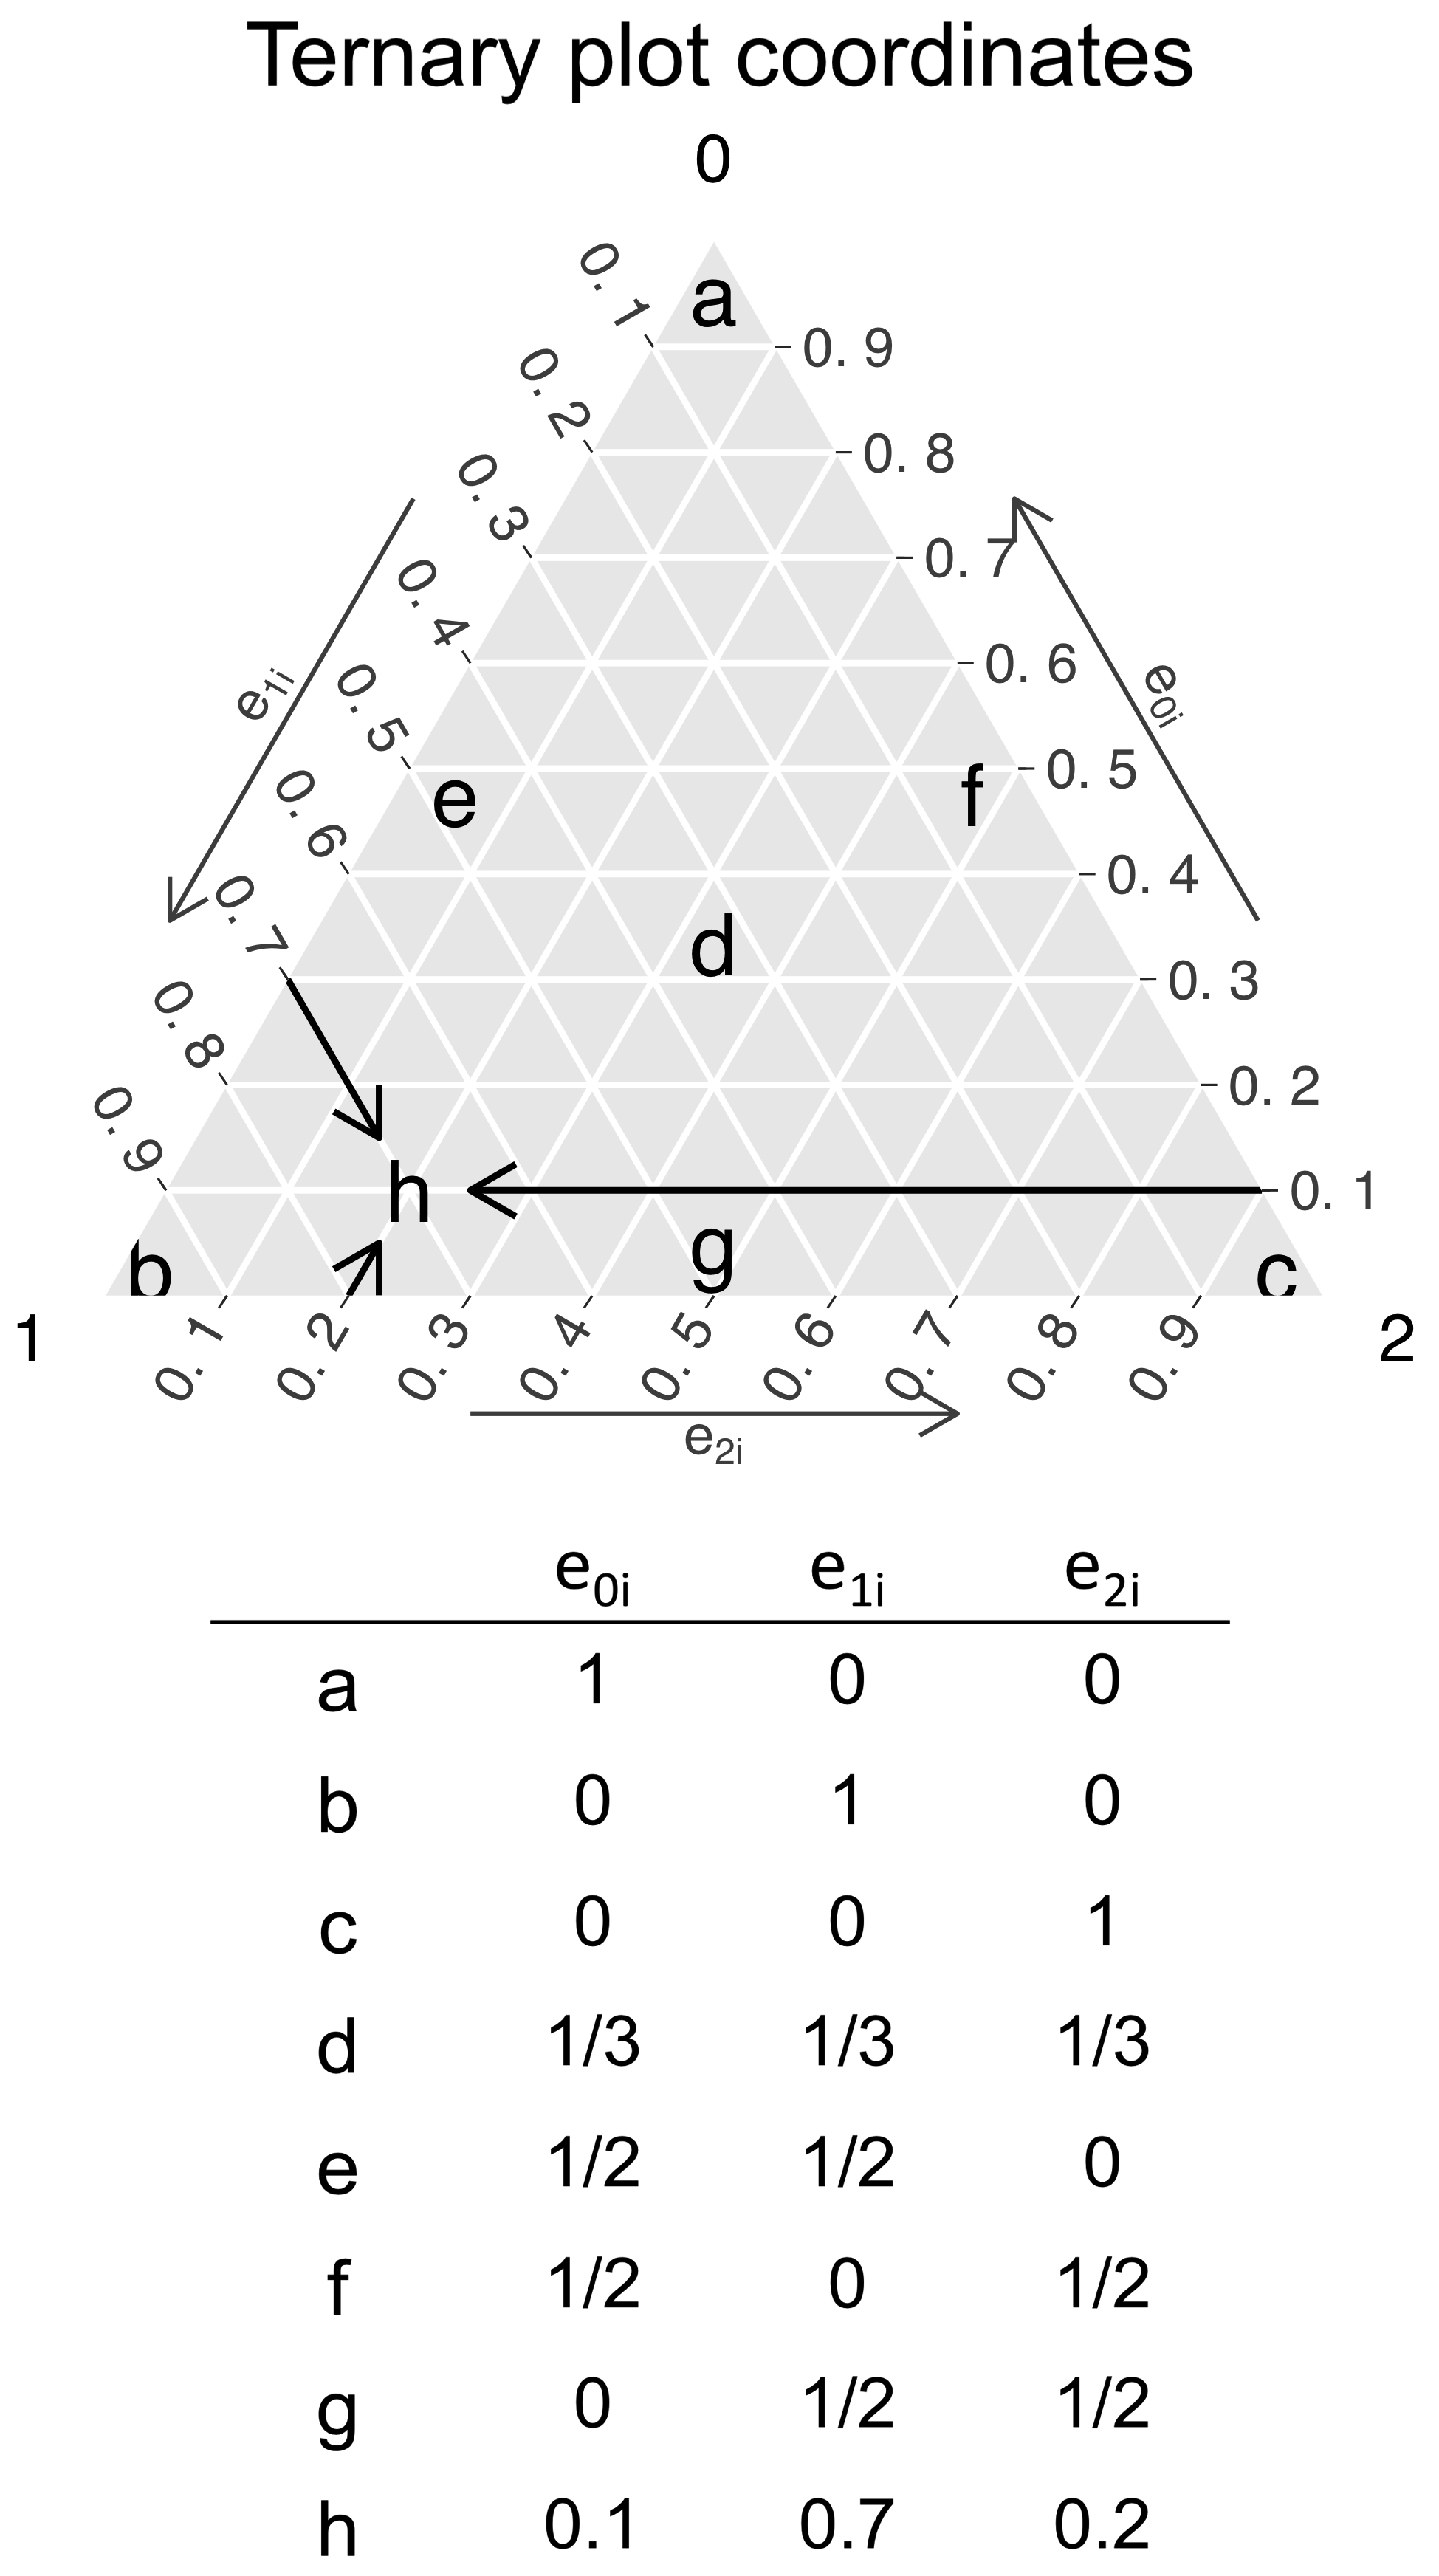
\includegraphics[page=1,keepaspectratio,width=1.0\textwidth]{../lib/ternary_coordinate_and_table_trimmed.png}
\end{center}
\end{column}
\end{columns}
\end{exampleblock}

\begin{exampleblock}{}
\large
\begin{itemize}
\item When the groups were similar in patient characteristics as expected in NSAIDs examples, most people were kept in the cohort after trimming.
\item Stürmer's and Walker's methods adapted to the skewness in the distributions due to marginal prevalence of treatments.
\end{itemize}
\end{exampleblock}
\end{block}

\begin{block}{Simulation Study}
\large
\begin{itemize}
\item We conducted simulation to examine bias reduction by trimming in settings in which the tails of PS distributions had unmeasured confounders.
\end{itemize}

\vspace{-2cm}
\begin{exampleblock}{}
\begin{columns}
\begin{column}{0.7\columnwidth}
\begin{center}
\includegraphics[page=2,keepaspectratio,width=1.0\textwidth,height=1.0\textheight]{../../../_trimming_stats/code/out/bias.pdf}
\end{center}
\end{column}

\begin{column}{0.3\columnwidth}
\tiny
\begin{align*}
  &\text{Measured covariates}\\
  \bX_{i}^{m} &= \begin{bmatrix}
    X_{1i} & X_{2i} & X_{3i} & X_{4i} & X_{5i} & X_{6i} \\
  \end{bmatrix}^{T}\\
  &\text{Unmeasured covariates}\\
  \bX_{i}^{u} &= \begin{bmatrix}
    X_{7i} & X_{8i} & X_{9i}\\
  \end{bmatrix}^{T}
\end{align*}

\scriptsize
\begin{center}
  \begin{tikzpicture}[%
    ->,
    shorten >=2pt,
    >=stealth,
    node distance=1cm,
    pil/.style={
      ->,
      thick,
      shorten =2pt,}
    ]
    %% Nodes
    \node (Xm) {$\bX^{m}_{i}$};
    \node[below = 0.3cm of Xm] (Xu) {$\bX^{u}_{i}$};
    \node[below left  = 2cm and 1.5cm of Xm] (A) {$A_i$};
    \node[below right = 2cm and 1.5cm of Xm] (Y) {$Y_i$};
    %% Xm to Xu Effect Association
    \draw[very thick] (Xm) -> (Xu);
    %% Treatment Effect Association
    \draw[very thick] (A) -> (Y);
    %% Confounder-Exposure Association
    \draw[very thick] (Xu) -> (A);
    \draw[very thick] (Xm) -> (A);
    %% Confounder-Outcome Association
    \draw[very thick] (Xu) -> (Y);
    \draw[very thick] (Xm) -> (Y);
  \end{tikzpicture}
\end{center}
\tiny
The unmeasured confounders were made more prevalent in the three tails of the PS distribution. \(A_{i}\) was a three-valued treatment and \(Y_{i}\) was a Poisson outcome.\\
~\\

\tiny
\alert{X-axis}: increasing level of trimming\\
\alert{Y-axis}: bias on the log rate ratio scale (zero is unbiased)\\
~\\
\alert{1vs0}: Group 1 vs Group 0\\
\alert{2vs0}: Group 2 vs Group 0\\
\alert{2vs1}: Group 2 vs Group 1\\
~\\
\alert{Unadj}: Unadjusted\\
\alert{IPTW}: Inverse probability of treatment weights\\
\alert{MW}: Matching weights \cite{YoshidaMatchingWeightsSimultaneously2017}\\
\alert{OW}: Overlap weights \cite{LiBalancingCovariatesPropensity2016}\\
\end{column}
\end{columns}
\end{exampleblock}

\begin{exampleblock}{}
\begin{itemize}
\item Bias was reduced by all methods, but Stürmer's and Walker's methods reduced bias more successfully when group sizes were highly imbalanced.
\item All methods reduced variance of the IPTW estimator, but not MW and OW estimators.
\end{itemize}
\end{exampleblock}
\end{block}

\begin{block}{Conclusions}
\begin{itemize}
\item We proposed a multinomial extension of the existing two-group PS trimming methods.

\item The extensions of Stürmer and Walker’s PS trimming methods reduced bias in 3-group exposure settings even with highly imbalanced treatment frequencies (10:10:80).

\item Examining how effect estimates vary at different trimming thresholds can be a useful sensitivity analysis although roles of treatment effect heterogeneity may also need consideration.
\end{itemize}
\end{block}

\begin{block}{Bibliography}
\vspace{-0.7ex}
\scriptsize
\renewcommand{\section}[2]{}
\bibliographystyle{apalike}
\bibliography{../../../../../../.emacs.d/misc/zotero}
\end{block}
\end{column}
\end{columns}
\end{frame}
\end{document}